%! TeX program = lualatex
\documentclass[12pt,a4paper]{article}

\usepackage[nil]{babel}
\usepackage{unicode-math}
\usepackage[svgnames]{xcolor}
\usepackage{lmodern}
\usepackage{graphicx}
\usepackage{wrapfig}
\usepackage{float}
\usepackage{parskip}
\usepackage[font=small,labelfont=bf]{caption}
\usepackage{hyperref}


\babelprovide[import=el, main, onchar=ids fonts]{greek} % can also do import=el-polyton
\babelprovide[import, onchar=ids fonts]{english}

\babelfont{rm}
          [Language=Default]{Liberation Sans}
\babelfont[english]{rm}
          [Language=Default]{Liberation Sans}
\babelfont{sf}
          [Language=Default]{Liberation Sans}
\babelfont{tt}
          [Language=Default]{Liberation Sans}

%Enter Title Here
 \title{Team-plan-v1.0 \\ LibShare}
 \author{\textbf{Ονόματα / ΑΜ / Έτος:} \\ Γρηγόρης Καπαδούκας / 1072484 / 4\textdegree \\ Χρήστος Μπεστητζάνος / 1072615 / 4\textdegree \\ Νικόλαος Αυγέρης / 1067508 / 5\textdegree \\ Περικλής Κοροντζής / 1072563 / 4\textdegree\\ \href{https://github.com/GregKapadoukas/University-Software-Engineering-Project}{\color{blue}GitHub Link}}
\begin{document}

\makeatletter
\begin{center}
	\LARGE{\@title} \\
	\pagebreak
    \begin{LARGE}\@author\end{LARGE}
\pagebreak
\end{center}

%Insert Body Here
\section{Χρονοπρογραμματισμός του project}
Με σκοπό τον χρονοπρογραμματισμό του project και την εκτίμηση της εργασίας που θα κάνουμε ως ομάδα, έχουμε αρχικά χωρίσει το project σε επιμέρους tasks.

Επίσης έχουμε ορίσει τις ημερομηνίες και τη διάρκεια σε μέρες που θα ασχοληθούμε με το κάθε task (ημερομηνία τέλους - ημερομηνία έναρξης = χρόνος κανονικής εκτίμησης). Ακόμα έχουμε υπολογίσει εξαρτήσεις μεταξύ των task, με τη μορφή του immediate predecessor.

Οι πληροφορίες αυτές που εκτιμήσαμε και αναφέρονται παραπάνω, παρουσιάζονται στον πίνακα στο Σχήμα \ref{Πίνακας Χρονοπρογραμματισμού Project}.

\begin{figure}[H]
	\makebox[\textwidth]{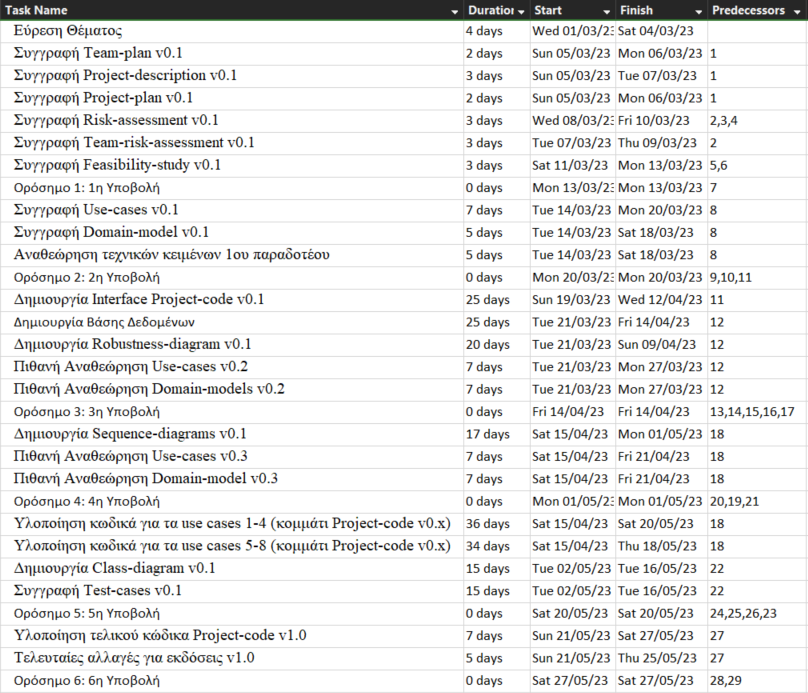
\includegraphics[width=\textwidth]{Team-Plan Table.png}}
	\caption{Πίνακας Χρονοπρογραμματισμού Project}
	\label{Πίνακας Χρονοπρογραμματισμού Project}
\end{figure}

Σημειώνω ότι έχουμε κάνει και εκτιμήσεις για χρόνους χειρότερης και καλύτερης περίπτωσης, τους οποίους με συνδυασμό με τους χρόνους κανονικής εκτίμησης χρησιμοποιούμε για να υπολογίσουμε τον μέσο χρόνο (αναμενόμενη διάρκεια) και τη διασπορά για κάθε task. Παραπάνω για τις εκτιμήσεις και τους υπολογισμούς αυτούς στην ενότητα \ref{Ενότητα Pert Chart} (συγκεκριμένα στο Σχήμα \ref{Πίνακας Pert Data}).

Τέλος σημειώνω ότι έχει γίνει και ανάθεση εργασίας στα μέλη της ομάδας η οποία παρουσιάζεται στην ενότητα \ref{Ενότητα Gantt Chart} (πιο συγκεκριμένα στο Σχήμα \ref{Gantt Chart Χρονοπρογραμματισμού Project}).

\subsection{Gantt chart}
\label{Ενότητα Gantt Chart}
Χρησιμοποιώντας τα δεδομένα του πίνακα από το Σχήμα 1 δημιουργήσαμε Gantt chart που απεικονίζει ποιες ημέρες και για πόσο μεγάλο χρονικό περιθώριο εκτιμούμε ότι θα ασχοληθούμε με το κάθε Task. Το Gantt chart αυτό απαρτίζει το Σχήμα \ref{Gantt Chart Χρονοπρογραμματισμού Project}.

\begin{figure}[H]
	\makebox[\textwidth]{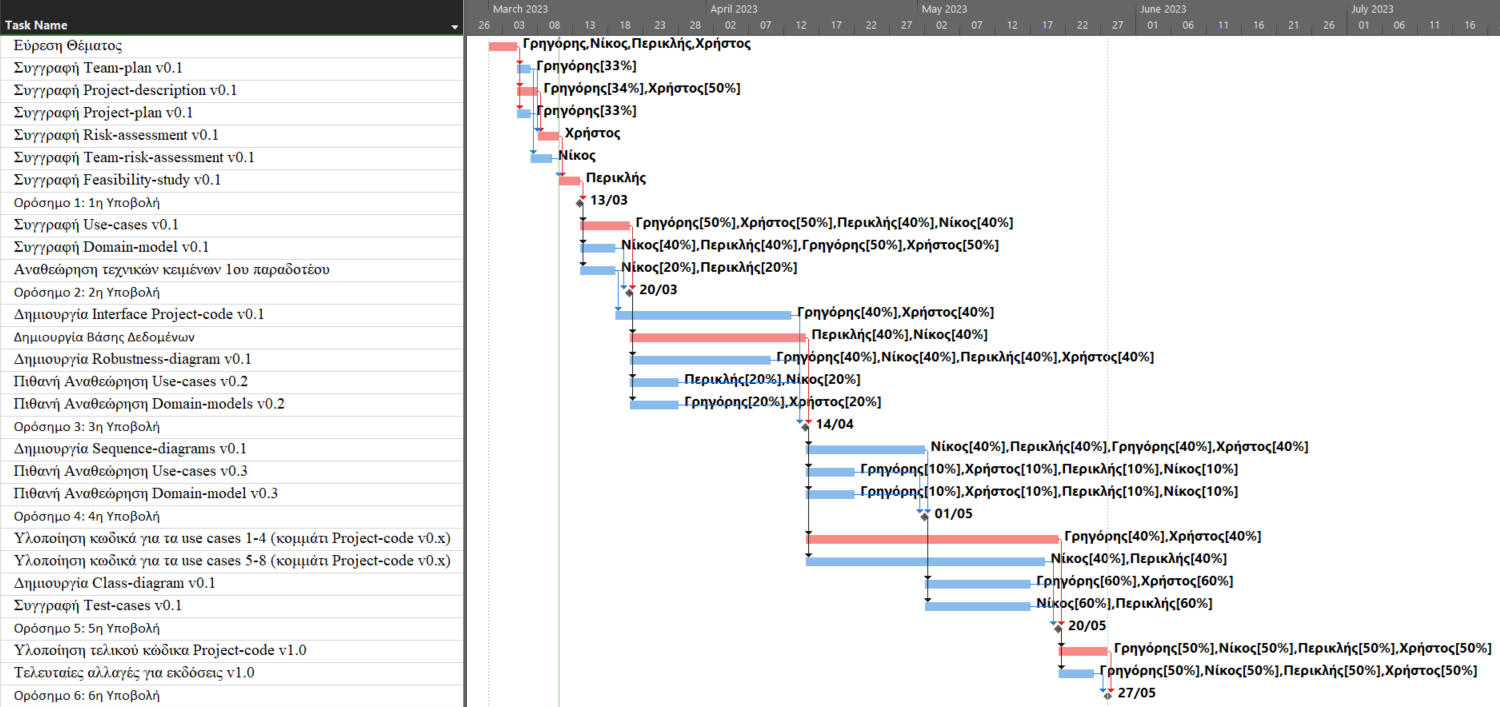
\includegraphics[width=\textwidth]{Team-Plan Gantt.png}}
	\caption{Gantt Chart Χρονοπρογραμματισμού Project}
	\label{Gantt Chart Χρονοπρογραμματισμού Project}
\end{figure}

Στην αριστερή στήλη φαίνονται τα ονόματα από τα task που αποσκοπούν σε κάθε bar του Gantt chart. Οπότε το κάθε όνομα είναι στην ίδια γραμμή με το bar που του αντιστοιχεί.

Σημειώνουμε ότι στο Gantt διάγραμμα παρουσιάζουμε επίσης ποια μέλη της ομάδας ορίσαμε υπεύθυνα για την διεκπεραίωση κάθε task (ανάθεση εργασίας). Οπότε δίπλα από κάθε bar παρουσιάζεται ένα ή παραπάνω ονόματα, μαζί με ένα ποσοστό για κάθε άτομο που δείχνει το ποσοστό του χρόνου του που θα αφοσιωθεί σε αυτό το task κατά τη διάρκεια διεκπεραίωσής του.

Τέλος με κόκκινο χρώμα παραπάνω συμβολίζεται το κρίσιμο μονοπάτι για το Gantt chart. Αντίστοιχα με μπλε χρώμα είναι τα μη κρίσιμα μονοπάτια. Σημειώνουμε εδώ ότι υπολογίζοντας τους χρόνους κανονικής εκτίμησης προέκυψε απευθείας ένα και μοναδικό κρίσιμο μονοπάτι, οπότε δεν χρειάστηκε να χρησιμοποιηθεί η διασπορά για την εκτίμηση για την εύρεση του κρίσιμου μονοπατιού, παρόλα αυτά έχουμε και πάλι συμπεριλάβει υπολογισμούς διασποράς και αναμενόμενης διάρκειας στο Σχήμα \ref{Πίνακας Pert Data}.


\subsection{Pert chart}
\label{Ενότητα Pert Chart}
Χρησιμοποιώντας τα δεδομένα από το Σχήμα \ref{Πίνακας Χρονοπρογραμματισμού Project}, φτιάχνουμε Pert chart (Σχήμα \ref{Pert Chart Χρονοπρογραμματισμού Project}) που απεικονίζει τα task μαζί με τις εξαρτήσεις που προκύπτουν μεταξύ των tasks.

\textbf{Σημείωση:} Για να χωρέσει το σχήμα στη σελίδα αναγκαστήκαμε να το συρρικνώσουμε αρκετά, με αποτέλεσμα τα γράμματα να είναι πολύ μικρά. Παρόλα αυτά παρατηρούμε πως μέσω λειτουργίας zoom αυτά φαίνονται. Αν παρόλα αυτά επιθυμείτε να προβάλλεται τα διαγράμματα με μεγαλύτερη ανάλυση, υπάρχουν αναρτημένα στο GitHub repository στον φάκελο "1ο Παραδοτέο/Team-Plan/v0.2/Files" σε μορφή .pptx καθώς και σε .png (screenshot). Επίσης δίνουμε τα στοιχεία του Pert chart στο συνοδευτικό πίνακα στο Σχήμα \ref{Πίνακας Pert Data} ακριβώς από κάτω, συμπληρωμένο με τιμές διακύμανσης και αναμενόμενης διάρκειας (δεν χρειάστηκαν βέβαια για να υπολογίσουμε το κρίσιμο μονοπάτι).

Εδώ με κόκκινο χρώμα συμβολίζεται το κρίσιμο μονοπάτι και με μαύρο συμβολίζονται τα μη κρίσιμα μονοπάτια.

\begin{figure}[H]
	\makebox[\textwidth]{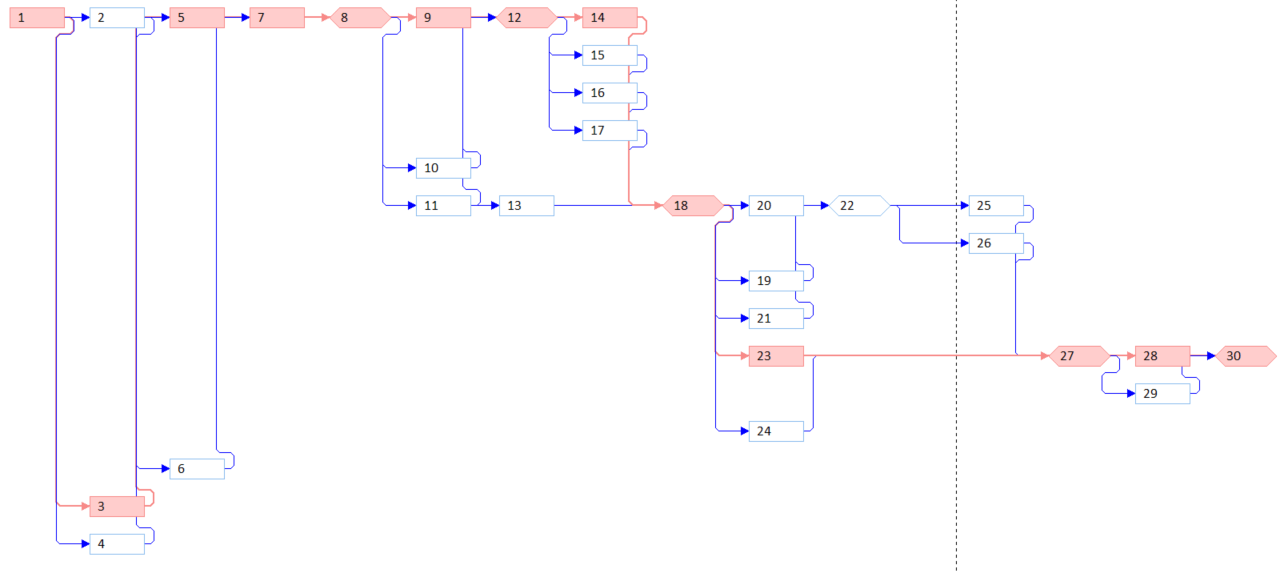
\includegraphics[width=\textwidth]{Team-Plan Pert.png}}
	\caption{Pert Chart Χρονοπρογραμματισμού Project}
	\label{Pert Chart Χρονοπρογραμματισμού Project}
\end{figure}

\begin{figure}[H]
	\makebox[\textwidth]{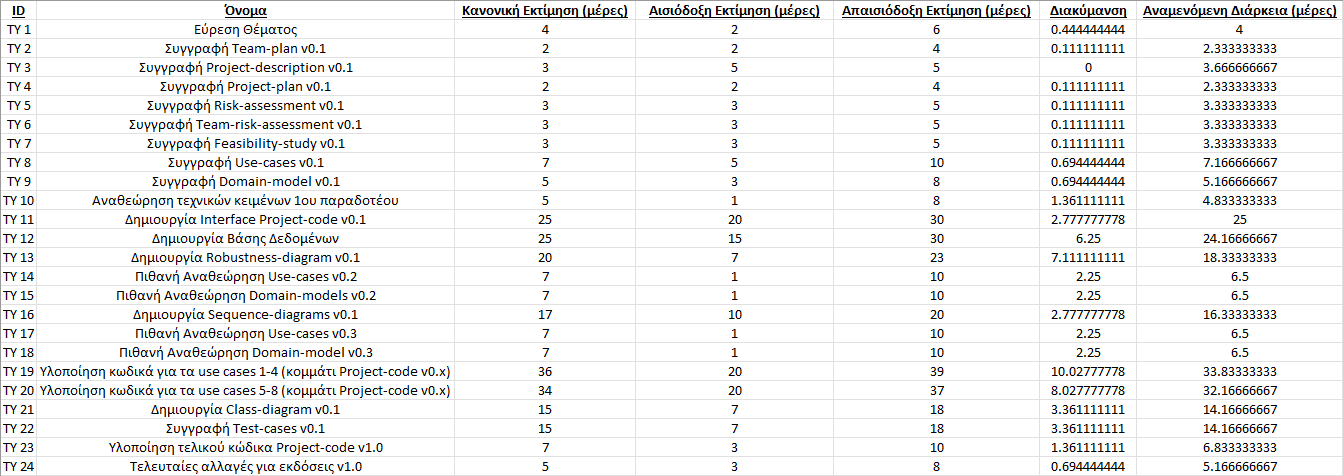
\includegraphics[width=\textwidth]{Team-Plan Pert Data.png}}
	\caption{Πίνακας Pert Data}
	\label{Πίνακας Pert Data}
\end{figure}


\section{Οργάνωσης Ομάδας}

\subsection{Μέθοδος Οργάνωσης}
Κατά τον χρονοπρογραμματισμό της εργασίας προσέξαμε ότι, μέσω της ανάθεσης της δουλειάς που παρουσιάζουμε στο Σχήμα \ref{Gantt Chart Χρονοπρογραμματισμού Project}, έχουμε γενικά μια καλή γνώση της εργασίας που θα πρέπει να κάνει το κάθε μέλος σε κάθε χρονική στιγμή. 

Παρόλα αυτά όμως, μερικά tasks όπως αυτά που αποσκοπούν στη συγγραφή κώδικα, είναι πολύ high level και θα είναι ιδανικό να υποδιαιρεθούν σε επιμέρους υπό tasks. Αποφασίσαμε λοιπόν ότι για την υλοποίηση αυτών των tasks θα χρησιμοποιήσουμε προσαρμοσμένη μέθοδο Scrum.

Με αυτόν τον τρόπο κάθε task που αποσκοπεί σε συγγραφή κώδικα, ανατίθεται σε ένα sprint που θα υλοποιείται αντίστοιχα από τα άτομα που το έχουν αναλάβει στο Σχήμα \ref{Gantt Chart Χρονοπρογραμματισμού Project}. Έτσι μπορούμε να χωριζόμαστε σε υπό ομάδες και μπορούμε να έχουμε πολλαπλά sprints σε εξέλιξη ταυτόχρονα, στις περιπτώσεις που αυτό βγάζει νόημα (πχ υλοποίηση βάσης και user interface μαζί).

Βέβαια θα υπάρχει επικοινωνία μεταξύ των υπό ομάδων και του Scrum Master που θα συντονίζει τις ομάδες και είναι υπεύθυνος για τον σχεδιασμό κάθε sprint cycle και των product backlog, με σκοπό την μετέπειτα ομαλή διασύνδεση της δουλειάς μεταξύ ομάδων ή/και με τη προηγούμενη δουλειά. Ο Scrum Master θεωρείται επίσης μέλος των ομάδων και γράφει κώδικα, όπως τα υπόλοιπα μέλη.

Έχουμε επιπλέον ορίσει εβδομαδιαίο Scrum meeting εξ αποστάσεως κάθε Πέμπτη στις 8:30 μμ. Με το meeting αυτό επιθυμούμε να κρατάμε επαφή, να επιλύουμε απορίες και να ανταλλάσσουμε ιδέες πάνω σε αυτά που ασχολούμαστε. Έχουμε επίσης ορίσει εναλλακτικές / επιπρόσθετες μέρες συνάντησης στην έκτακτη περίπτωση που κάποιο μέλος δεν μπορεί να προσέλθει την Πέμπτη ή που κρίνουμε ότι χρειαζόμαστε πάνω από ένα meeting, να είναι το Σάββατο στις 3 μμ ή / και τη Δευτέρα στις 9:30 μμ. Τέλος υπολογίζουμε το ενδεχόμενο να προσθέσουμε ακόμα παραπάνω συναντήσεις στη βδομάδα αν αυτό απαιτείται.

\subsection{Ρόλοι Μελών Ομάδας}

\begin{enumerate}
	\item \textbf{Γρηγόρης Καπαδούκας:} Product Owner, Scrum Master, Editor,\\ Tester, Peer Reviewer, Programmer.
	\item \textbf{Χρήστος Μπεστητζάνος:} Product Owner, Editor, Peer Reviewer, Tester, UX Designer, Programmer.
	\item \textbf{Νικόλαος Αυγέρης:} Editor, Peer Reviewer, Database Designer,\\ Tester, Programmer
	\item \textbf{Περικλής Κοροντζής:} Editor, Peer Reviewer, Analyst, Tester, Programmer
\end{enumerate}

Σημειώνουμε ότι σκοπός είναι να ασχοληθούμε όλοι με κάθε ρόλο, αν και οι παραπάνω ρόλοι λειτουργούν ενδεικτικά για τα ζητήματα με τα οποία θα ασχοληθούν κατά κόρον τα μέλη της ομάδας. Επισημαίνεται επίσης ότι οι όροι Product Owner και Scrum Master συμπεριλήφθηκαν λόγω της ανάγκης ύπαρξης τους από τις προδιαγραφές του Scrum. Ως Product Owner ορίσαμε τα άτομα που επινόησαν την ιδέα του έργου και έγραψαν το Project-description.

\section{Βασικά Εργαλεία που Χρησιμοποιήσαμε}
\label{Βασικά Εργαλεία που Χρησιμοποιήσαμε}

\subsection{Συγγραφή Κειμένων}
Για τη συγγραφή των τεχνικών κειμένων χρησιμοποιούμε LaTeX, με χρήση του engine LuaTex (άρα LuaLaTeX). Τα .tex αρχεία της εργασίας περιέχονται επίσης στο GitHub της εργασίας.

\subsection{Γλώσσα Προγραμματισμού και Περιβάλλον Ανάπτυξης Λογισμικού}
Σκοπεύουμε να χρησιμοποιήσουμε μια αντικειμενοστραφή προσέγγιση με Python 3 για την ανάπτυξη του λογισμικού, με χρήση της βιβλιοθήκης CustomTKinter για το GUI, επειδή πιστεύουμε πως η ευκολία χρήσης και εκμάθησης των λειτουργιών της σαν γλώσσα θα μας βοηθήσει πολύ να υλοποιήσουμε αποδοτικά το έργο.

Το περιβάλλον ανάπτυξης λογισμικού που θα χρησιμοποιηθεί κατά κόρον είναι το Visual Studio Code της Microsoft, αν και τα μέλη της ομάδας θα έχουν την ευχέρεια να χρησιμοποιήσουν άλλα εργαλεία αν θέλουν όπως PyCharm και Neovim, με την προϋπόθεση βέβαια ότι ο τελικός κώδικας θα ελεγχτεί να λειτουργεί σε όλες τις εφαρμογές που αναφέρονται.

\subsection{Σχεδιασμός Σχημάτων, Mock-up Screens και Charts}
Θα χρησιμοποιηθεί ένας συνδυασμός από εργαλεία, όπως Paint, Paint.net, Microsoft Excel, Microsoft Project, Microsoft PowerPoint, Visual Paradigm, Gimp, Figma κ.α. Επειδή τα μέλη της ομάδας έχουν διαφορετικό βαθμό εξοικείωσης με διάφορα εργαλεία που θέλουμε να αξιοποιήσουμε. Προϋπόθεση πάντα βέβαια της χρήσης ενός εργαλείου είναι να υπάρχει μια ομοιομορφία με τα υπόλοιπα σχήματα και γραφήματα που έχουν ήδη χρησιμοποιηθεί.

\section{Εμπλούτιση Κειμένου για τη Τελευταία Έκδοση}
\label{Final Chapter}

\subsection{Κατανομή Προσπάθειας της Ομάδας}

\begin{itemize}
    \item \textbf{Γρηγόρης Καπαδούκας:} Ε\textsubscript{1} = 
	\item \textbf{Χρήστος Μπεστητζάνος:} Ε\textsubscript{2} = 
	\item \textbf{Νικόλαος Αυγέρης:} Ε\textsubscript{3} =  
	\item \textbf{Περικλής Κοροντζής:} Ε\textsubscript{4} =  
\end{itemize}

\subsection{Τελικό Gantt Chart και Ανάθεση Έργου}

\subsection{Συμπεράσματα από τον Τρόπο Εργασίας ως Ομάδα}

\subsubsection{Αλλαγές που προέκυψαν στο τρόπο συνεργασίας}

Σχετικά με τον τρόπο συνεργασίας ως ομάδα, παρατηρήσαμε αρχικά ότι ορισμένες από τις ιδέες και προδιαγραφές του SCRUM δεν μας φάνηκαν τόσο ωφέλιμες για ομάδα μόνο τεσσάρων ατόμων, οπότε δεν εφαρμόστηκαν με την αυστηρή έννοια των προδιαγραφών που ορίσαμε.

Έτσι για παράδειγμα, δεν έγινε σχεδιασμός και χρήση product backlog, με την έννοια που γίνεται κανονικά σε ομάδες που χρησιμοποιούν SCRUM, παρά είχαμε τον ίδιο τον Scrum Master υπεύθυνο για την συντήρηση μιας λίστας από tasks που έπρεπε να γίνουν για κάθε παραδοτέο, και στις ομαδικές συναντήσεις γινόταν ομαδική συμφωνία καταχώρησης των tasks σε διαφορετικά μέλη της ομάδας και συμφωνία καταληκτικών ημερομηνιών όπου έπρεπε ο καθένας να έχει τελειώσει τη δουλειά που ανέλαβε και διαμοιραζόταν εκ νέου εργασία.

Επίσης τελικά καταλήξαμε να μην ορίζουμε sprints γύρω από τα tasks του κώδικα, με τον τρόπο που αναφέρεται παραπάνω, αλλά τα sprint cycles μας ήταν βασισμένα πάνω στις προθεσμίες υποβολών του κάθε παραδοτέου. Άρα είχαμε ένα sprint cycle για κάθε υποβολή, που δεν περιείχε φάση ανάλυσης, σχεδίασης, υλοποίησης, εφαρμογής και αξιολόγησης, παρά ασχολούμασταν με τις φάσεις στις οποίες αποσκοπούσε το κάθε παραδοτέο κάθε φορά, και στις φάσεις που αποσκοπούσαν τα προηγούμενα παραδοτέα όταν κάναμε διορθώσεις τους.

Ακόμα αναφέρουμε ότι δεν είχαμε σταθερή δομή χωρισμό της ομάδας σε μικρότερες ομάδες των δύο μελών τελικά, παρά δουλεύαμε ο καθένας ανεξάρτητα στη δουλειά που του είχε ανατεθεί κάθε φορά, με συχνή επικοινωνία με τον Scrum Master για τυχόν βοήθεια ή επίλυση αποριών και μέσω των συναντήσεων γινόταν παρουσίαση της δουλειάς του κάθε ατόμου κάθε φορά και δινόταν feedback από όλα τα μέλη της ομάδας.

Τέλος αναφέρουμε ότι ο ρόλος του Scrum Master δεν κατάντησε τελικά να τον εναλλάσσουμε μεταξύ των μελών των ομάδων ανά παραδοτέο, αλλά τον είχε ο Γρηγόρης Καπαδούκας για όλη τη διάρκεια της εργασίας. Με αυτό το τρόπο κρατήσαμε μια σταθερότητα στις ευθύνες που είχε κάθε άτομο της ομάδας για τη διάρκεια της εργασίας και μπορέσαμε με το καιρό να βελτιώνουμε την απόδοση των μελών, χωρίς την ανάγκη για προσαρμογή σε νέους ρόλους σε κάθε sprint.

\subsubsection{Συμπεράσματα}

Σημειώνουμε πως με τις αλλαγές στον τρόπο συνεργασίας που κάναμε, νιώθουμε ότι η μέθοδος που χρησιμοποιήσαμε μας βοήθησε για τον συντονισμό των μελών, εφόσον γνωρίσαμε όλοι σε κάθε χρονική στιγμή τι έπρεπε να γίνει από τον καθένα μας και σε τι χρονικό διάστημα, χωρίς να γίνεται διπλότυπη εργασία και χωρίς να δημιουργούνται παρεξηγήσεις για το ποιο άτομο είναι υπεύθυνο για κάποιο task.

Αν μπορούσαμε να γυρίσουμε το χρόνο πίσω, θα επιμέναμε παραπάνω στα αρχικά χρονοδιαγράμματά μας, συγκεκριμένα στο ξεκίνημα συγγραφής του κώδικα νωρίτερα, όπως σκοπεύαμε αρχικά αλλά δεν καταφέραμε να κάνουμε. Αυτό το αναφέρουμε επειδή η εμπειρία που αποκτήσαμε κατά τη συγγραφή του κώδικα μας βοήθησε πολύ να εντοπίσουμε και να διορθώσουμε λάθη στη σχεδίαση που είχαμε κάνει, τα οποία αν είχαμε νωρίτερα την εμπειρία αυτή δεν θα τα είχαμε κάνει εξαρχής.


\section{Συμμετοχή και Ρόλοι στη Συγγραφή του Κειμένου}
\begin{enumerate}
	\item \textbf{Γρηγόρης Καπαδούκας:} Author
	\item \textbf{Χρήστος Μπεστητζάνος:} Editor, Contributor
	\item \textbf{Νικόλαος Αυγέρης:} Peer Reviewer
	\item \textbf{Περικλής Κοροντζής:} Peer Reviewer
\end{enumerate}

\section{Αλλαγές από έκδοση σε έκδοση}

\subsection{Από έκδοση v0.1 σε έκδοση v0.2}
\begin{itemize}
    \item Αλλαγή του χρονοπρογραμματισμού και της ανάθεσης εργασίας ώστε να αποσκοπούν παραπάνω αυτό που έγινε στη πραγματικότητα.
    \item Ανανέωση του Gantt chart ώστε να είναι πιο ευδιάκριτες οι ημερομηνίες.
    \item Ανανέωση του Pert ώστε να περιέχει τα στοιχεία, εφόσον ενημερωθήκαμε πως δεν ήταν επαρκής ο συνοδευτικός πίνακας του v0.1.
    \item Προσθήκη της Τρίτης ως μέρας συναντήσεων
    \item Προσθήκη του Microsoft PowerPoint και Figma στα εργαλεία που χρησιμοποιούμε.
\end{itemize}

\subsection{Από έκδοση v0.2 σε έκδοση v1.0}
\begin{itemize}
    \item Ανανέωση του κειμένου "\ref{Βασικά Εργαλεία που Χρησιμοποιήσαμε} Βασικά Εργαλεία που Χρησιμοποιήσαμε".
    \item Προσθήκη κεφαλαίου "\ref{Final Chapter}: Εμπλούτιση Κειμένου για τη Τελευταία Έκδοση".
\end{itemize}

\end{document}
